%! Author = drakanoy
%! Date = 10.09.2024

% Preamble
\documentclass[12pt]{article}

% Packages
\usepackage[utf8]{inputenc}
\usepackage[T2A]{fontenc}
\usepackage[english, russian]{babel}
\usepackage[a4paper, includefoot, left=1.5cm, right=1.5cm, top=1cm, bottom=1.5cm, headsep=1cm, footskip=1cm]{geometry}
\usepackage{makecell}
\usepackage{amsmath}
\usepackage{graphicx}
\usepackage{enumitem}
\usepackage{svg}
\usepackage{multirow}
\usepackage{hyperref}
\usepackage{mathtools}
\usepackage{amssymb}
\usepackage{textcomp}
\usepackage{stmaryrd}

% Document
\begin{document}
\begin{large}
\begin{center}
\LARGE \textbf{Домашняя работа}
\par
\LARGE \textbf{Кононов Александр Михайлович}
\par
    \textbf{26.12.2024}
\end{center}
\par Условие:
\par
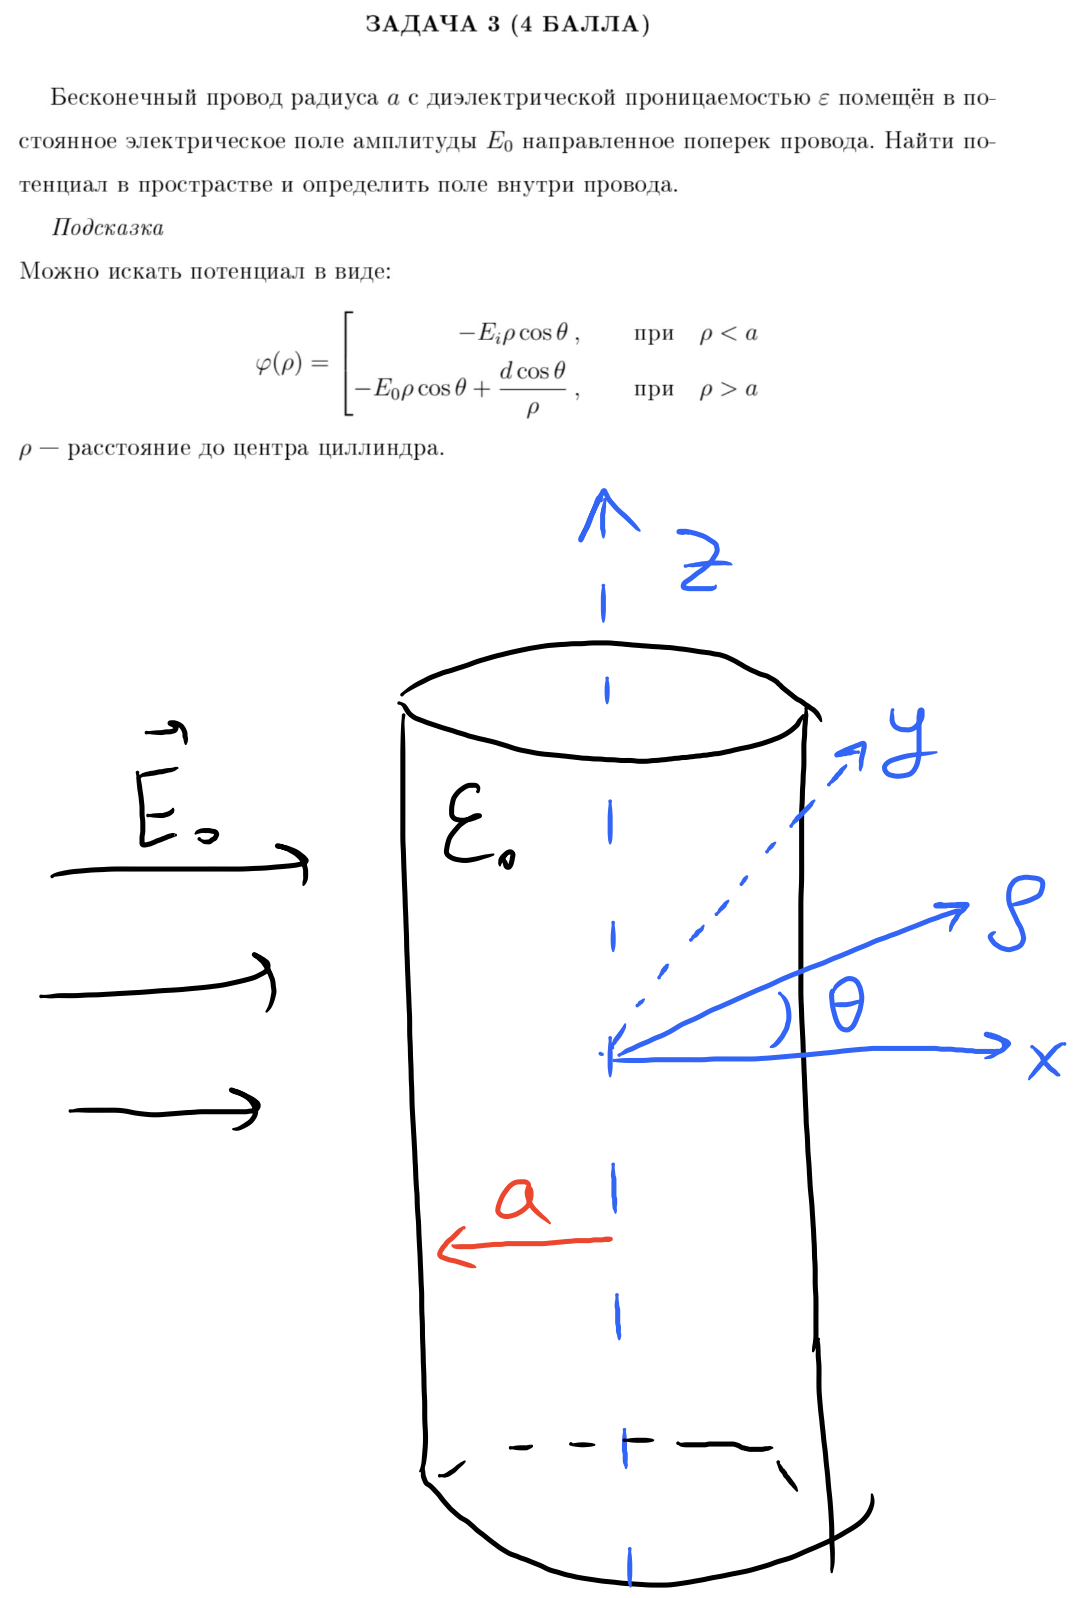
\includegraphics[width=0.8\textwidth]{photo.png}
%\begin{center}
%\underline{Рисунок 1}:
%\end{center}
\par Решение:
\par
\par
%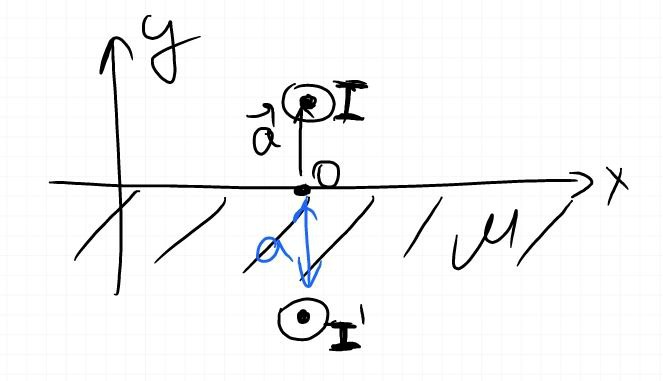
\includegraphics[width=1\textwidth]{photo_1.jpg}
%\par
%\begin{center}
%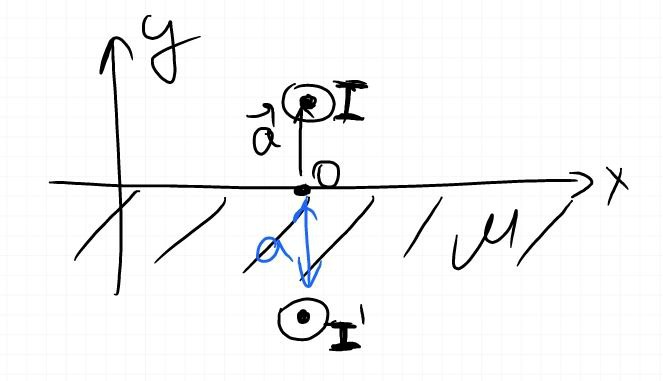
\includegraphics[width=0.4\textwidth]{photo_1.jpg}
%\end{center}
\[
    \overrightarrow{E}_{seat} \left( \vec{r} \right) = \widehat{G} \left( \vec{r} \right) \vec{p}
\]
\[
    \vec{p} = \alpha_x E_{0x} \vec{e_x} + \alpha_y E_{0y} \vec{e_y}
\]
\[
    G_{\alpha \beta } = \left( q^2 \delta_{\alpha \beta} + \frac{\partial }{\partial x_\alpha}\frac{\partial }{\partial x_\beta} \right) \frac{e^{iqr}}{r} ;  \, \, \, \alpha; \beta = x; y; z
\]
\par так как $r >> 1/q$:
\[
    G_{\alpha \beta } = \frac{1}{r} \left( q^2 \delta_{\alpha \beta} + \frac{\partial }{\partial x_\alpha}\frac{\partial }{\partial x_\beta} \right)e^{iqr} = q^2 \left( \delta_{\alpha \beta} + n_\alpha n_\beta \right) \frac{e^{iqr}}{r}
\]
\[
    E_i = G_{ij}\left( \alpha_j E_{0j} \right) ;  \, \, \, i; j = x; y; z
\]
\par Пусть пока $|E_{0x}|^2 + |E_{0y}|^2 = I$
\begin{eqnarray*}
    \begin{cases}
        \xi_1 = \frac{1}{I}\left( E_{0x}E_{0y}^* + E_{0x}^*E_{0y} \right) = \frac{2}{I} Re\left( E_{0x}E_{0y}^* \right) = 2|E_{0x}||E_{0y}| \cos \delta ; \,\,\, \delta - \text{Разность фаз} \\
        \xi_2 = \frac{1}{I i}\left( E_{0x}E_{0y}^* - E_{0x}^*E_{0y} \right) = \frac{2}{I} Im\left( E_{0x}E_{0y}^* \right) = 2|E_{0x}||E_{0y}| \sin \delta \\
        \xi_3 = \frac{1}{I} \left( |E_{0x}|^2 - |E_{0y}|^2 \right)
    \end{cases}
\end{eqnarray*}
\par Из условия
\begin{eqnarray*}
    \begin{cases}
        \xi_1 = 0 \Rightarrow \cos \delta = 0  \Rightarrow \sin \delta = 1 \\
        \xi_2 = 24/25 \Rightarrow |E_{0x}||E_{0y}| = \frac{12}{25}I \\
        \xi_3 = -7/25 \Rightarrow |E_{0x}|^2 - |E_{0y}|^2 = -\frac{7}{25}I
    \end{cases}
\end{eqnarray*}
\begin{eqnarray*}
    \Rightarrow
    \begin{cases}
        |E_{0x}| = \frac{3}{5}\sqrt{I} \\
        |E_{0y}| = \frac{4}{5}\sqrt{I}
    \end{cases}
    \Rightarrow
    \begin{cases}
        E_{0x} = |E_{0x}| e^{i \pi /2} = |E_{0x}| \cdot i\\
        E_{0y} = |E_{0y}|
    \end{cases}
\end{eqnarray*}
\par Такое определение $\xi_1; \xi_2; \xi_3$ - когда мы смотрим на падующую волну. То есть ее волновой вектор направлен на нас. В таком случае в сферической сисетме коореднат мы их переопределим через замену $E_x \shortrightarrow E_\varphi ; E_y \shortrightarrow - E_\theta $
\par Найдем новые $ E_x; E_y; E_z $, после этого найдем $E_\theta ; E_\varphi$, и тогда найдем вектора Стокса.
\[
    E_i = G_{ij}\left( \alpha_j E_{0j} \right) ;  \, \, \, i; j = x; y; z
\]
\begin{equation*}
    \begin{pmatrix}
        E_x \\
        E_y \\
        E_z
    \end{pmatrix}
    =
    \begin{pmatrix}
        1 - n_x^2 & -n_x n_y &  -n_x n_z\\
        -n_y n_x & 1 - n_y^2 &  -n_y n_z\\
        -n_z n_x & -n_z n_y &  1 - n_z^2
    \end{pmatrix}
    \begin{pmatrix}
        \alpha_x E_{0x} \\
        \alpha_y E_{0y} \\
        0
    \end{pmatrix}
    \cdot q^2 \frac{e^{iqr}}{r}
\end{equation*}
\begin{equation*}
    \begin{pmatrix}
        E_x \\
        E_y \\
        E_z
    \end{pmatrix}
    =
    \begin{pmatrix}
        \alpha_x E_{0x} - n_x^2 \alpha_x E_{0x} - n_x n_y \alpha_y E_{0y} \\
        \alpha_y E_{0y} - n_y^2 \alpha_y E_{0y} - n_x n_y \alpha_x E_{0x} \\
        - n_x n_z \alpha_x E_{0x} - n_y n_z \alpha_y E_{0y}
    \end{pmatrix}
    \cdot q^2 \frac{e^{iqr}}{r}
\end{equation*}
\par Выразим $n_x; n_y; n_z$ через $n_r; n_\theta; n_\varphi$. Так как мы всегда будем смотреть по $n_r$, то $n_\theta = n_\varphi = 0; n_r = 1$. Это по сути переход из декартовых коореднат в сферические
\begin{eqnarray*}
    \begin{cases}
        n_x = \sin \theta \cos \varphi \\
        n_y = \sin \theta \sin \varphi \\
        n_z = \cos \theta
    \end{cases}
\end{eqnarray*}
\begin{equation*}
    \begin{pmatrix}
        E_x \\
        E_y \\
        E_z
    \end{pmatrix}
    =
    \begin{pmatrix}
        \alpha_x E_{0x} - \sin^2 \theta \cos^2 \varphi \alpha_x E_{0x} - \sin^2 \theta \sin \varphi \cos \varphi \alpha_y E_{0y} \\
        \alpha_y E_{0y} - \sin^2 \theta \sin^2 \varphi \alpha_y E_{0y} - \sin^2 \theta \sin \varphi \cos \varphi \alpha_x E_{0x} \\
        - \sin \theta \cos \theta \cos \varphi \alpha_x E_{0x} - \sin \theta \cos \theta \sin \varphi \alpha_y E_{0y}
    \end{pmatrix}
    \cdot q^2 \frac{e^{iqr}}{r}
\end{equation*}
\par Переходим в сферические коорденаты:
\begin{equation*}
    \begin{pmatrix}
        E_r \\
        E_\theta \\
        E_\varphi
    \end{pmatrix}
    =
    \begin{pmatrix}
        \sin \theta \cos \varphi & \sin \theta \sin \varphi & \cos \theta\\
        \cos \theta \cos \varphi & \cos \theta \sin \varphi & -\sin \theta\\
        -\sin \varphi & \cos \varphi & 0
    \end{pmatrix} \times
\end{equation*}
\begin{equation*}
    \times
    \begin{pmatrix}
        \alpha_x E_{0x} - \sin^2 \theta \cos^2 \varphi \alpha_x E_{0x} - \sin^2 \theta \sin \varphi \cos \varphi \alpha_y E_{0y} \\
        \alpha_y E_{0y} - \sin^2 \theta \sin^2 \varphi \alpha_y E_{0y} - \sin^2 \theta \sin \varphi \cos \varphi \alpha_x E_{0x} \\
        - \sin \theta \cos \theta \cos \varphi \alpha_x E_{0x} - \sin \theta \cos \theta \sin \varphi \alpha_y E_{0y}
    \end{pmatrix}
    \cdot q^2 \frac{e^{iqr}}{r}
\end{equation*}
\par Магия математики:
\begin{equation*}
    \begin{pmatrix}
        E_r \\
        E_\theta \\
        E_\varphi
    \end{pmatrix}
    =
    \begin{pmatrix}
        0 \\
        \cos \theta \left( \alpha_x E_{0x} \cos \varphi + \alpha_y E_{0y} \sin \varphi \right) \\
        \alpha_y E_{0y} \cos \varphi - \alpha_x E_{0x} \sin \varphi
    \end{pmatrix}
    \cdot q^2 \frac{e^{iqr}}{r}
\end{equation*}
\begin{eqnarray*}
\Rightarrow
    \begin{cases}
        \xi_1 = - \frac{2 Re\left( E_\theta E_\varphi^* \right)}{|E_\theta|^2 + |E_\varphi|^2} \\
        \xi_2 = - \frac{2 Im\left( E_\theta E_\varphi^* \right)}{|E_\theta|^2 + |E_\varphi|^2} \\
        \xi_3 = \frac{|E_\theta|^2 - |E_\varphi|^2}{|E_\theta|^2 + |E_\varphi|^2} \\
    \end{cases}
\end{eqnarray*}
\par Подаставляем $E_r; E_\theta; E_\varphi$, учитываем $E_{0x} = |E_{0x}| i ; E_{0y} = |E_{0y}|$, получаем:
\begin{eqnarray*}
    \begin{cases}
        \xi_1 = \frac{2 \cos \theta \left( \alpha_y^2 |E_{0y}|^2 - \alpha_x^2 |E_{0x}|^2 \right) \cos \varphi \sin \varphi}{\left( \cos^2 \theta + 1 \right)\left( \alpha_y^2 |E_{0y}|^2 \varphi + \alpha_x^2 |E_{0x}|^2 \cos \varphi \right)} \\
        \xi_2 = \frac{2 \cos \theta \alpha_x |E_{0x}| \alpha_y |E_{0y}| \left( \cos^2 \varphi + \sin^2 \varphi \right)}{\left( \cos^2 \theta + 1 \right)\left( \alpha_y^2 |E_{0y}|^2 \varphi + \alpha_x^2 |E_{0x}|^2 \cos \varphi \right)} \\
        \xi_3 = \frac{\cos^2 \theta - 1}{\cos^2 \theta + 1} = - \frac{\sin^2 \theta}{\cos^2 \theta + 1}
    \end{cases}
\end{eqnarray*}
\begin{eqnarray*}
    \begin{cases}
        \xi_1 = \frac{2 \cos \theta \left( \alpha_y^2 \frac{16}{25} - \alpha_x^2 \frac{9}{25} \right) \cos \varphi \sin \varphi}{\left( \cos^2 \theta + 1 \right)\left( \alpha_y^2 \frac{16}{25} \varphi + \alpha_x^2 \frac{9}{25} \cos \varphi \right)} \\
        \xi_2 = \frac{2 \cos \theta \alpha_x \alpha_y \frac{4}{5} \frac{3}{5}}{\left( \cos^2 \theta + 1 \right)\left( \alpha_y^2 |E_{0y}|^2 \varphi + \alpha_x^2 |E_{0x}|^2 \cos \varphi \right)} \\
        \xi_3 = - \frac{\sin^2 \theta}{\cos^2 \theta + 1}
    \end{cases}
\end{eqnarray*}
\par Теперь $\alpha_x; \alpha_y$
\par Приблизим нашу фигуру Элипсоидом вращения. В такмо случае полуоси:
\[
    a_x = h; a_y = a_z = R
\]
\par В таком случае в литературе (Г. ван де Хюлст 'Рассеяние света малыми частицами' , параграф 6.3) находим выражения для $\alpha_i$
\par
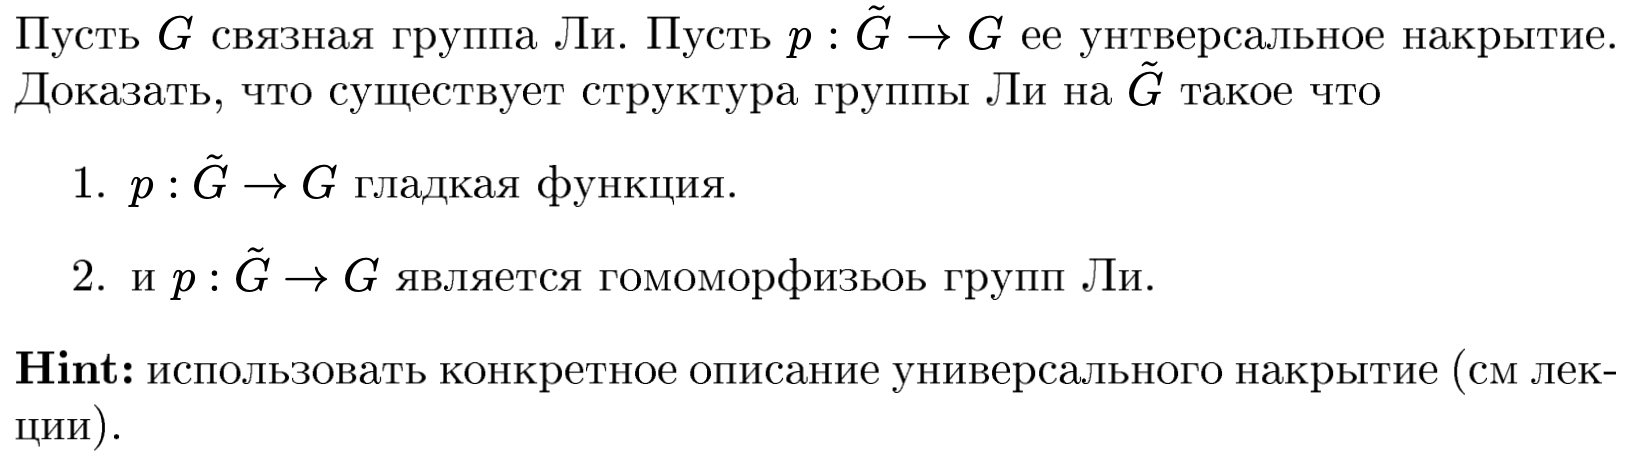
\includegraphics[width=1\textwidth]{photo_2.png}
\par
\[
    \alpha_i = \frac{V \left( \varepsilon - 1 \right)}{1 + \left( \varepsilon - 1 \right) N_i}
\]
\[
    V = \frac{4}{3}\pi R^2 h
\]
\[
    V = \frac{4}{3}\pi R^2 h
\]
\[
    N_x = \frac{1-e^2}{e^3}\left( \frac{1}{2} \ln \frac{1+e}{1-e} - e \right) ; \, \, \, e = 1 - \frac{R^2}{h^2}
\]
\[
    N_y = N_z = \frac{1}{2} \left( 1 - N_x \right)
\]
\par Ответ:
\begin{eqnarray*}
    \begin{cases}
        \xi_1 = \frac{2 \cos \theta \left( \alpha_y^2 \frac{16}{25} - \alpha_x^2 \frac{9}{25} \right) \cos \varphi \sin \varphi}{\left( \cos^2 \theta + 1 \right)\left( \alpha_y^2 \frac{16}{25} \varphi + \alpha_x^2 \frac{9}{25} \cos \varphi \right)} \\
        \xi_2 = \frac{2 \cos \theta \alpha_x \alpha_y \frac{4}{5} \frac{3}{5}}{\left( \cos^2 \theta + 1 \right)\left( \alpha_y^2 |E_{0y}|^2 \varphi + \alpha_x^2 |E_{0x}|^2 \cos \varphi \right)} \\
        \xi_3 = - \frac{\sin^2 \theta}{\cos^2 \theta + 1}
    \end{cases}
\end{eqnarray*}
\[
    \alpha_i = \frac{V \left( \varepsilon - 1 \right)}{1 + \left( \varepsilon - 1 \right) N_i}
\]
\[
    V = \frac{4}{3}\pi R^2 h
\]
\[
    V = \frac{4}{3}\pi R^2 h
\]
\[
    N_x = \frac{1-e^2}{e^3}\left( \frac{1}{2} \ln \frac{1+e}{1-e} - e \right) ; \, \, \, e = 1 - \frac{R^2}{h^2}
\]
\[
    N_y = N_z = \frac{1}{2} \left( 1 - N_x \right)
\]
\par
\par
\end{large}
\end{document}
